\subsubsection{Glück} \label{glueck-4}



\todo[inline]{Verantwortlich: Minas}




Um das Glück-Szenario in einer VR-Umgebung zu verwirklichen, wurden sich für HDR-Panorama-Bilder entschieden, die in Unreal eine Umgebung bilden sollen. 
Der Grund weswegen die Bilder HDR und Panorama sein müssen, werden im Laufe dieses Kapitels erklärt. 
Außerdem wird eine Audio-Datei im Hintergrund abgespielt und ein Text eingeblendet, welches thematisch zum Bild passt. 
Die Grundidee stammt vom ersten Prototypen (Kapitel 7.3.1), welches nicht in einer VR-Umgebung gelöst wurde. 
In Kapitel 7.3.1 wurde zudem erklärt, weshalb und welche Audio-Datei im Hintergrund abgespielt wird, weshalb die Texte eingeblendet werden und was sich unter Glück verstehen lässt. \\

Insgesamt besteht das Glück-Szenario aus acht HDR-Panorama-Bilder für das Hauptszenario und ein HDR-Panorama-Bild für das Warm-Up-Szenario. 
Abbildung \ref{fig-glueck4} zeigt alle Bilder die genutzt werden und deren Texte (falls vorhanden). \\

\begin{figure}[H] \centering
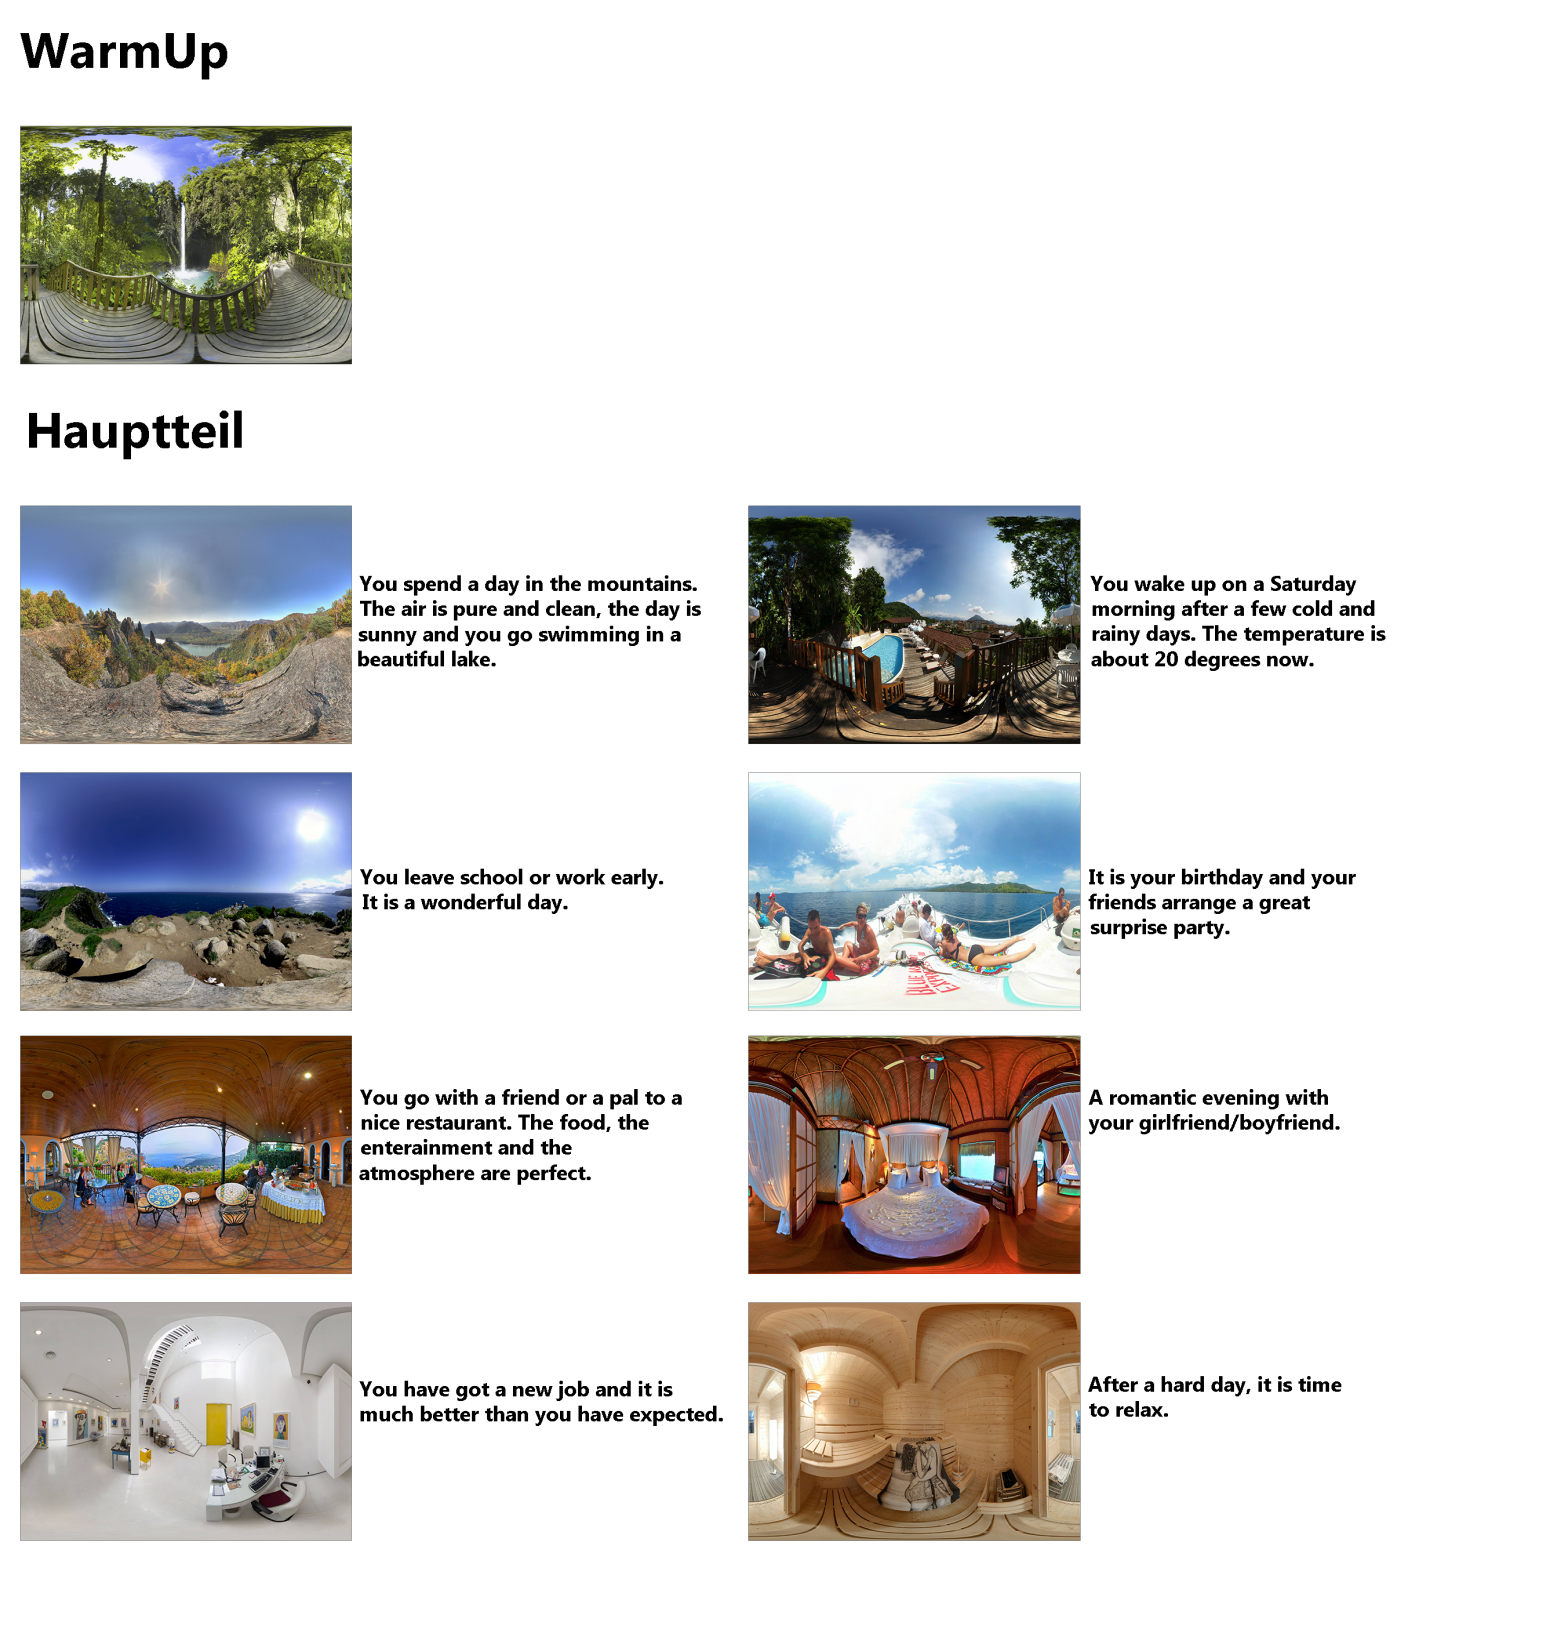
\includegraphics[width=15cm]{Images/gluck4.png} 
\vspace{-0.3cm} 
\caption[Im Glück-Szenario verwendete Bilder und deren Texte]{Im Glück-Szenario verwendete Bilder und deren Texte\cite{sun360}.}
\label{fig-glueck4} 
\end{figure}


Die Bilder lassen sich jedoch nicht ohne weiteres in Unreal einbinden. 
Um dies zu realisieren wurde sich für eine CubeMap in DDS-Format entschieden. 
Hierfür müssen die Bilder zunächst durch verschiedene Tools (Blender, Photoshop) bearbeitet werden und dann mit bestimmten Konfigurationen in Unreal eingebunden werden. \\

\begin{figure}[H] \centering
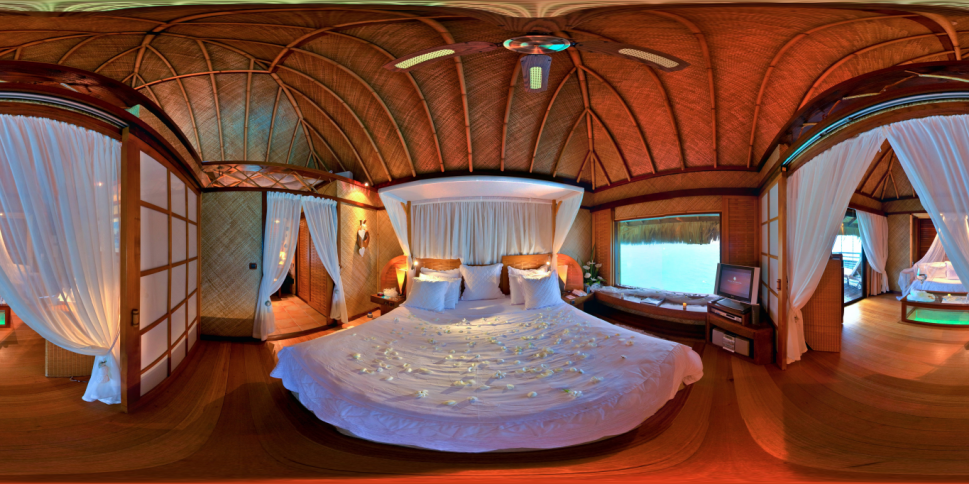
\includegraphics[width=\textwidth]{Images/hdr-panorama.png} 
\caption{Ein im Projekt verwendetes HDR-Panorama-Bild.}
\label{fig-hdr} 
\end{figure}


Anhand Abbildung \ref{fig-hdr} wird die Bearbeitung der Bilder erklärt. 
Nach Auswahl eines Panorma-HDR-Bildes, wird dieses in Blender bearbeitet. 
Blender wird benötigt, um aus dem gesamten Bild, sechs Einzelbilder mit der benötigten Rotation zu erzeugen. 
Das ist der erste Schritt um später eine CubeMap zu erzeugen. 
Im Internet existiert bereits eine Blender-File mit den benötigten Konfigurationen\cite{facerig19}, um an diese Einzelbilder zu gelangen. 
Diese besteht aus einer Kamera, welches um das importierte Bild rotiert und dieses zurecht schneidet. 
Handelt es sich um kein Panorama Bild, werden die sechs Bilder falsch geschnitten und können dadurch die Kriterien einer CubeMap nicht erfüllen. \\

\begin{figure}[H] \centering
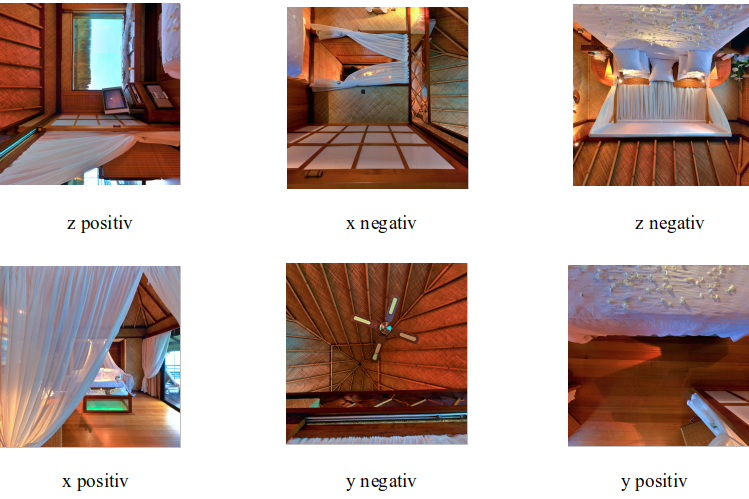
\includegraphics[width=\textwidth]{Images/blender-bilder.png} 
\caption{Ausgabe der Blender-File und deren Rotation.}
\label{fig-blender-bilder} 
\end{figure}


Um eine CubeMap in Unreal einzubinden, wird jedoch nur ein Bild im DDS-Format benötigt und nicht sechs Einzelbilder. 
DDS steht für Direct Draw Surface und ist ein entwickeltes Format von Microsoft. 
Dieses Format wird hauptsächlich für die Speicherung von CubeMaps und Texturen verwendet und erhöht die Geschwindigkeiten in Spielen ohne Verlust von Details\cite{dateiendungen19}.
Nvidia bietet ein Plugin für einige Adobe Photoshop Versionen und GIMP, um CubeMaps in DDS-Format abzuspeichern.
Der nächste Schritt eine CubeMap zu erstellen, wurde mit Adobe Photoshop CS2 und dem Nvidia Texture- Plugin realisiert. 
Hierfür müssen die Bilder in Abbildung \ref{fig-blender-bilder} in richtiger Reihenfolge aneinander gereiht werden. 
Dies geschieht in Adobe Photoshop. 
Die benötigte Reihenfolge wird in Abbildung \ref{fig-rotation} gezeigt. \\

\begin{figure}[H] \centering
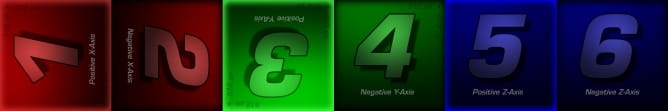
\includegraphics[width=\textwidth]{Images/rotation.png} 
\caption[Rotation und Reihenfolge für eine CubeMap]{Rotation und Reihenfolge für eine CubeMap\cite{franczak19}.}
\label{fig-rotation} 
\end{figure}


Somit ergibt sich für die Bearbeitung der Abbildung \ref{fig-blender-bilder}, Abbildung \ref{fig-blender-bilder2}. \\

\begin{figure}[H] \centering
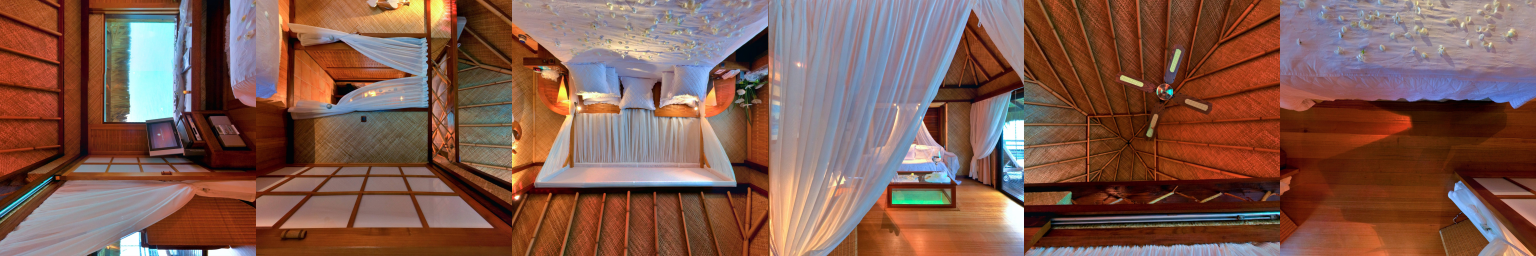
\includegraphics[width=\textwidth]{Images/blender-bilder2.png} 
\caption{Rotation und Reihenfolge für die CubeMap der Abbildung \ref{fig-blender-bilder}.}
\label{fig-blender-bilder2} 
\end{figure}


Nach einer aneinander Reihung der einzelnen Bilder, lässt sich das dadurch entstandene Bild mit Hilfe des Nvidia Plugins in eine DDS-File exportieren. 
Somit wird die gewünschte Cubemap generiert.
Abbildung \ref{fig-cubemap} zeigt die aufgeklappte Form einer CubeMap.
Jetzt kann die DDS-File in Unreal importiert bzw. konfiguriert werden. \\

\begin{figure}[H] \centering
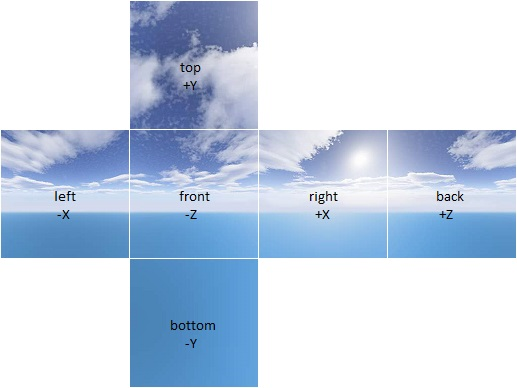
\includegraphics[width=\textwidth]{Images/cubemap.png} 
\caption[Aufgeklappte CubeMap]{Aufgeklappte CubeMap\cite{belanec19}.}
\label{fig-cubemap} 
\end{figure}


Sobald die DDS-File im Unreal-Projekt importiert wurde, muss an der DDS-File selbst Einstellungen vorgenommen werden. 
Abbildung \ref{fig-einstellungen} beinhaltet die optimalen Einstellungen. \\

\begin{figure}[H] \centering
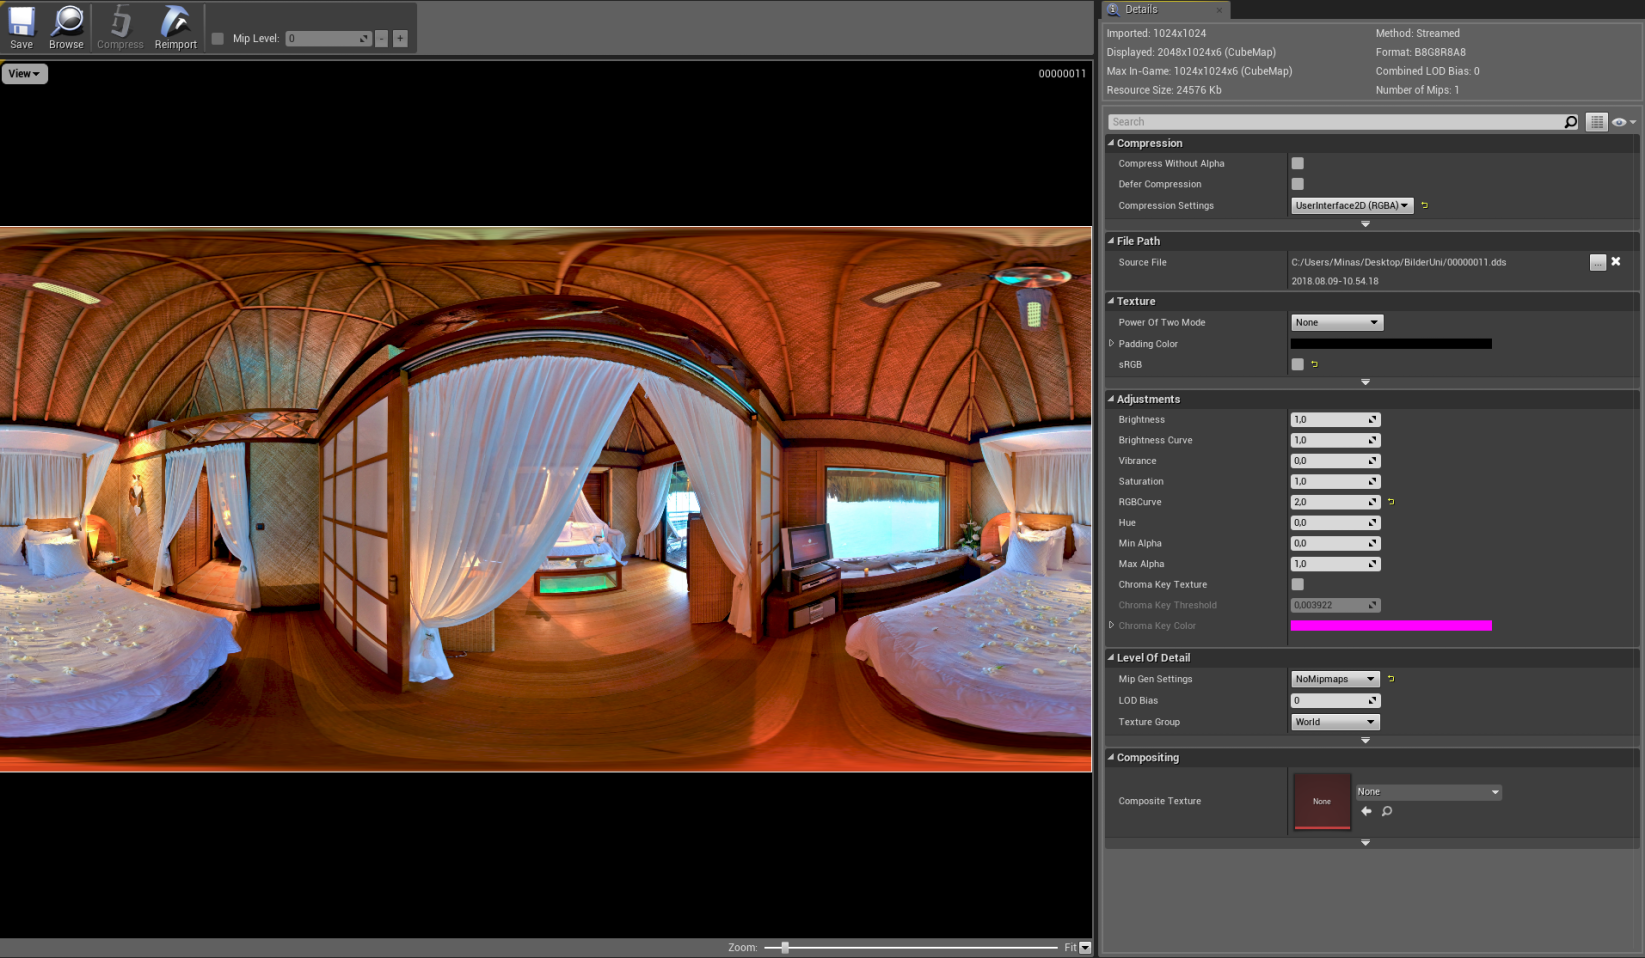
\includegraphics[width=\textwidth]{Images/einstellungen.png} 
\caption{Optimale Einstellungen des Bildes in Unreal.}
\label{fig-einstellungen} 
\end{figure}


Diese Einstellungen lassen sich für alle Bilder übernehmen. 
Lediglich die Einstellung RGBCurve unter ``Adjustments'' muss von Bild zu Bild variiert werden. 
Desto höher der eingetragene Wert, umso kräftiger werden die Farben des Bildes. 
Wird der Standardwert von ``1,0'' gelassen, wirkt das Bild sehr blass und ist damit nicht anschaulich. 
Hier spielt auch die Qualität des Bildes eine große Rolle. 
Am Anfang des Kapitels wurde HDR erwähnt. 
HDR steht für High Dynamic Range und ermöglicht ein größeren Helligkeitsbreich als SDR (Standard Dynamic Range). 
Es lässt das Bild realistischer wirken, ohne Farbtöne im dunklen oder hellen Bereichen zu vernachlässigen\cite{eizo19}.
Abbildung \ref{fig-sdr-hdr} zeigt den Qualitätsunterschied zwischen SDR und HDR.
Es ist von Vorteil ein solches Format zu verwenden, um eine gute VR-Umgebung zu realisieren. \\

\begin{figure}[H] \centering
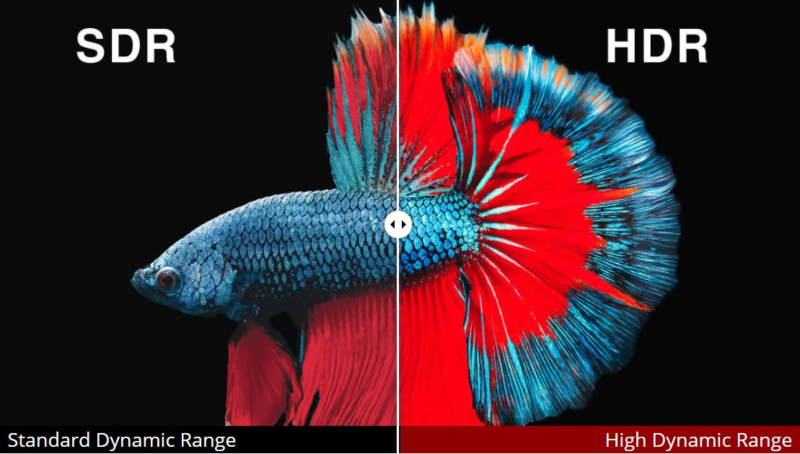
\includegraphics[width=8cm]{Images/sdr.png} 
\caption[SDR vs. HDR]{SDR vs. HDR\cite{finch19}.}
\label{fig-sdr-hdr} 
\end{figure}


Nach dem das Bild in Unreal fertig konfiguriert wurde, muss eine ``Blueprint Class'' angelegt werden. 
Diese wird in diesem Beispiel ``SkySphere-BP'' genannt. 
In diesem Blueprint wird eine Variable angelegt mit dem Namen ``SkyMaterial''. Außerdem sollte das Construction Script wie in Abbildung \ref{fig-skysphere} aufgebaut sein. \\

\begin{figure}[H] \centering
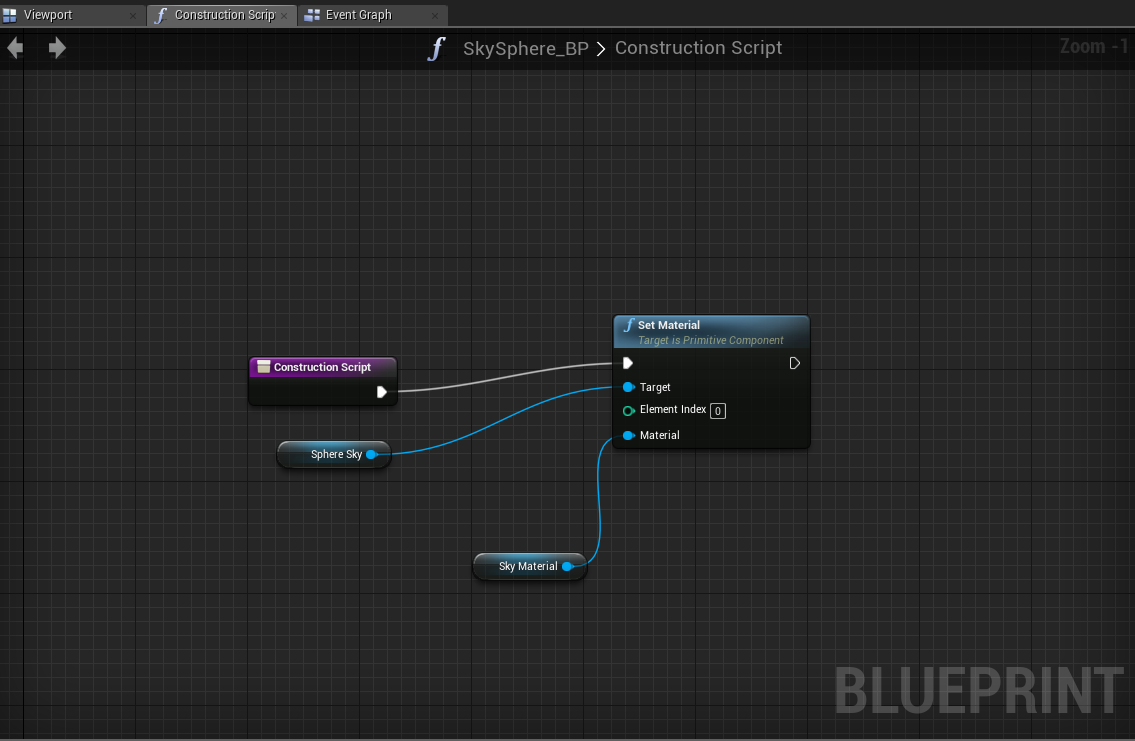
\includegraphics[width=8cm]{Images/skysphere.png} 
\caption{SkySphere-BP Construction Script.}
\label{fig-skysphere} 
\end{figure}


Mit diesem Construction Script lassen sich CubeMaps in die SkySphere importieren und bei Bedarf auch austauschen. \\

Nun muss ein Material für die SkySphere erstellt werden. Abbildung \ref{fig-konfiguration} zeigt wie diese Konfiguriert werden sollte. \\

\begin{figure}[H] \centering
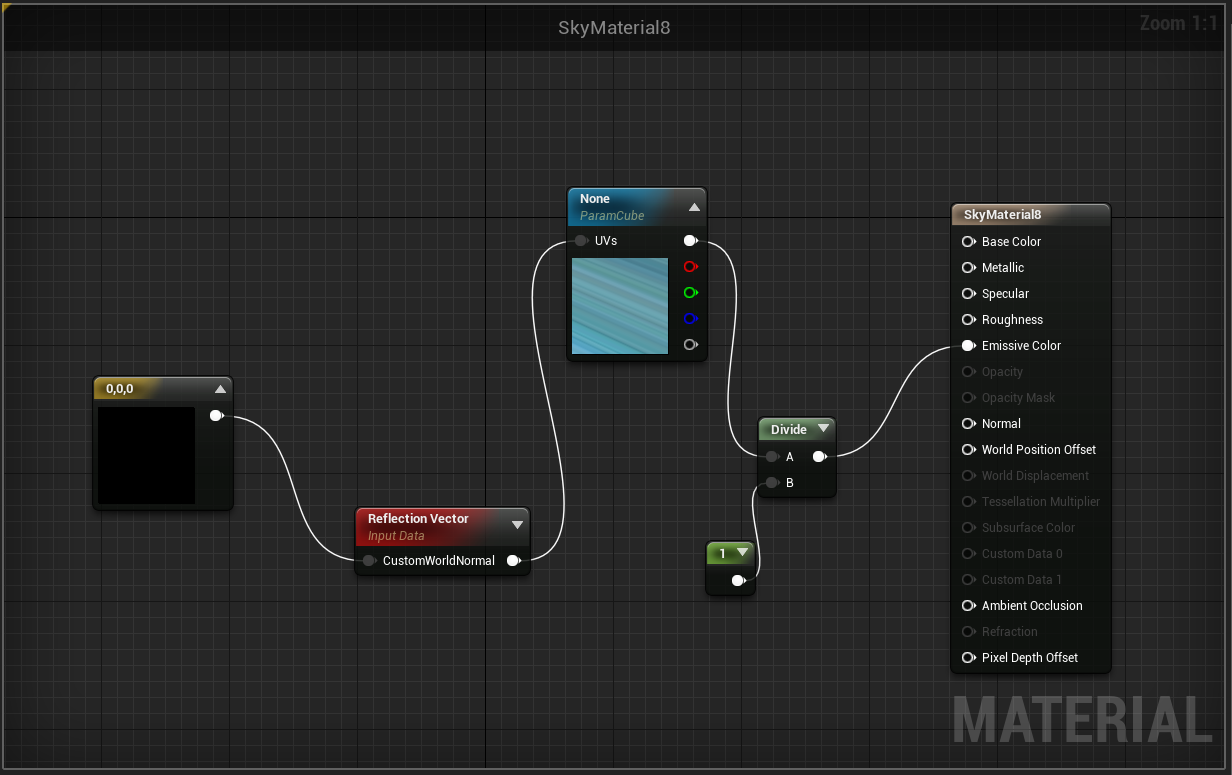
\includegraphics[width=8cm]{Images/konfiguration.png} 
\caption{Konfigurationen von Material.}
\label{fig-konfiguration} 
\end{figure}


Im Knoten ``ParamCube'' muss die Textur ausgesucht werden. 
In diesem Fall handelt es sich um die erstellte CubeMap. 
Als letztes muss das erzeugte Material der SkySphere zugewiesen werden. 
Nun lässt sich die Umgebung in Unreal anzeigen.
Der Text im Bild lässt sich mit einem Blueprint-Pawn erzeugen. 
Die Position des Textes wird manuell vorgenommen, in dem der Text im Bild verschoben wird. 
Damit der Übergang zwischen den Bildern angenehm für die Probanden wirken soll, wird ein ``fade in'' und ein ``fade out'' für jedes einzelne Bild erzeugt. 
Hierfür muss in Unreal unter Cinematics eine Matinee hinzugefügt werden. 
In dieser Matinee wird das Fade erzeugt, in dem die Anzeigedauer angegeben wird und vier Keys hinzugefügt werden. 
Der erste Key sagt dem Fade bei welcher Sekunde das Bild anfängt, der zweite Key bis wann das Bild seine maximale Helligkeit erreichen soll, der dritte Key ab wann das Bild wieder dunkler werden soll und der vierte Key bis wann das Bild komplett verschwunden sein soll. 
Abbildung \ref{fig-matinee} zeigt das Konfigurationsfenster der Matinee. \\

\begin{figure}[H] \centering
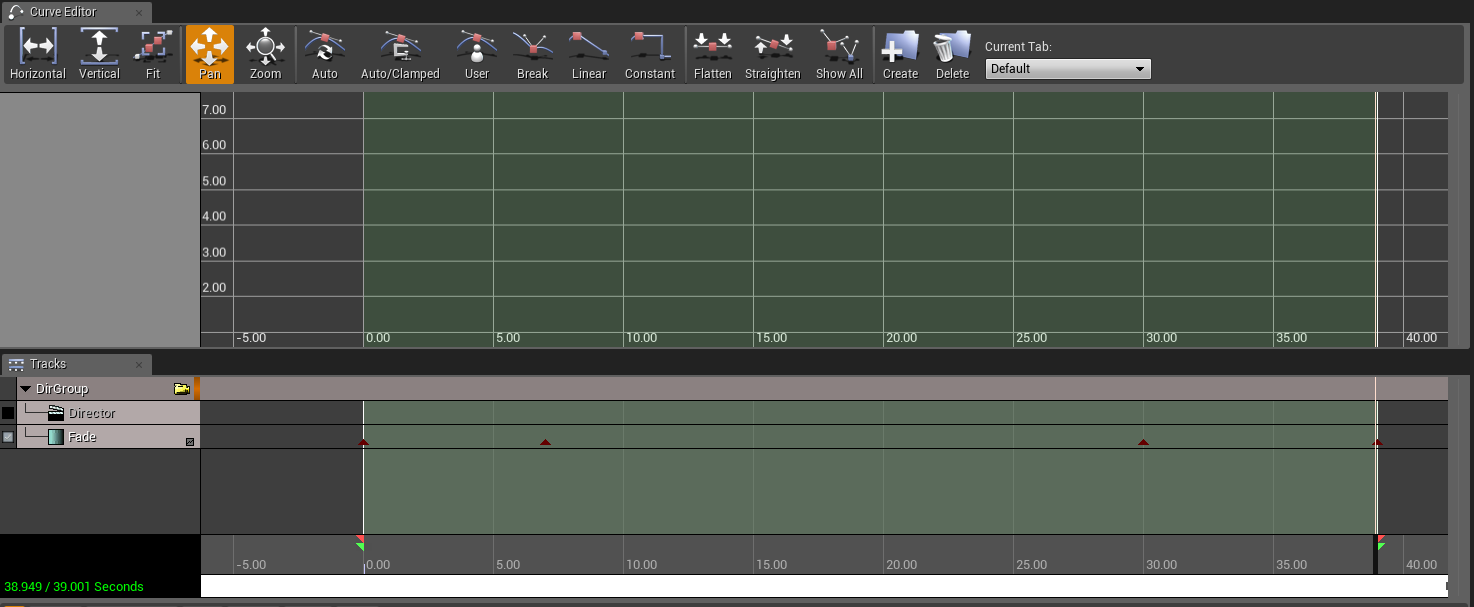
\includegraphics[width=\textwidth]{Images/matinee.png} 
\caption[Konfiguration der Matinee]{Konfiguration der Matinee; rote Dreiecke = Keys; grüner Bereich = Anzeigedauer.}
\label{fig-matinee} 
\end{figure}


Somit ist das erste Bild für das Szenario fertig konfiguriert. 
Dieser Ablauf wurde für acht weitere Bilder durchgeführt. \\

Der Wechsel zwischen den Bildern für das Hauptszenario wurde anhand der Level-Option von Unreal vorgenommen. 
Diese Option besteht aus einem anhaltenden Level und beliebig viele Level, die hinzugefügt werden können. 
In diesem Fall acht Level für die verwendeten Bilder. 
Das anhaltende Level beinhaltet die Audio-Datei und verwaltet den Wechsel der Bilder, welches alle 39 Sekunden durchgeführt wird. Die 39 Sekunden kamen zustande, in dem die Länge der Audio-Datei durch die Anzahl der Bilder geteilt wurde. 
Damit wurde vermieden das die Audio-Datei von Anfang an abgespielt wird. 
Ein großer Vorteil der Level-Option ist, dass die Audio-Datei fortläuft, auch während dem Level-Wechsel und somit keine Unterbrechungen entstehen. 
Da das WarmUp für das Glücks-Szenario nur aus einem Bild besteht, musste hier keine Level-Option konfiguriert werden. \\

